\documentclass[11pt]{article}
\usepackage[margin=2.3cm]{geometry}
\usepackage{tikz}
\pagestyle{empty}
\begin{document}
\begin{center}{\Large\bf B -- Fragile Bridges}\\[2pt]{\small Time limit: 2 seconds \quad Memory limit: 256 MB}\end{center}

The kingdom of Arcadia has $n$ islands connected by $m$ bidirectional bridges. A bridge is called
\emph{fragile} if removing it disconnects at least one pair of islands that were connected before.

\begin{center}
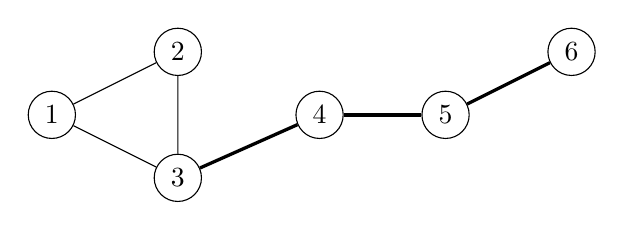
\begin{tikzpicture}[every node/.style={circle,draw,minimum size=6mm,inner sep=0pt}]
\node (1) at (0,0) {1}; \node (2) at (1.6,0.8) {2}; \node (3) at (1.6,-0.8) {3};
\node (4) at (3.4,0) {4}; \node (5) at (5.0,0) {5}; \node (6) at (6.6,0.8) {6};
\draw (1)--(2)--(3)--(1); \draw[very thick] (3)--(4); \draw[very thick] (4)--(5); \draw (5)--(6);
\draw[very thick] (5)--(6);
\end{tikzpicture}\\[2pt]
{\small Figure 1: the fragile bridges are drawn thicker.}
\end{center}

Given the map of the kingdom, find all fragile bridges. It is guaranteed that there is at most one
bridge between any pair of islands and that no bridge connects an island to itself.

\section*{Input}
The first line contains two integers $n$ and $m$ ($2 \le n \le 10^5$, $1 \le m \le 2 \cdot 10^5$).
Each of the next $m$ lines contains two integers $u_i$ and $v_i$ ($1 \le u_i, v_i \le n$), the islands
connected by the $i$-th bridge.

\section*{Output}
Print the number $k$ of fragile bridges. Then print $k$ lines, each with a pair $u$ $v$ ($u < v$)
describing a fragile bridge, sorted in lexicographic order. If there are none, print only \texttt{0}.

\section*{Sample Input}
\begin{verbatim}
6 7
1 2
2 3
3 1
3 4
4 5
5 6
\end{verbatim}

\section*{Sample Output}
\begin{verbatim}
3
3 4
4 5
5 6
\end{verbatim}
\end{document}
